
% \begin{document}

\chapter{SPSC Lockless Queue}

A single producer single consumer (SPSC) lockless queue is a data exchange queue
between a producer and a consumer. The SPSC lockless queue enables data exchange
between producer and consumer without the use of a lock, allowing both producer
and consumer to make progress in all scenarios.\\

An example application of an SPSC queue is a data exchange interface between the ASIC
and the CPU in a driver implementation.\\

A real implementation needs to account for memory ordering effects specific to
the architecture. For example, ARM has a weak memory ordering model where
read/write may appear out-of-order between CPUs. In this chapter, we will assume
\textit{logical} execution order where each command is perceived as issued
sequentially (even across CPUs) to focus the discussion on describing the system
using TLA+.

\section{Design}

The following describes the SPSC queue requirements: 

\begin{itemize}
      \item Two executing context, reader and writer
      \item Writer pointer advances after write 
      \item Reader pointer advances after reading      
      \item If read pointer equals write pointer, queue is empty
      \item If writer pointer + 1 equals read pointer, queue is full
\end{itemize}

The following is an example of an SPSC queue:
\begin{center}
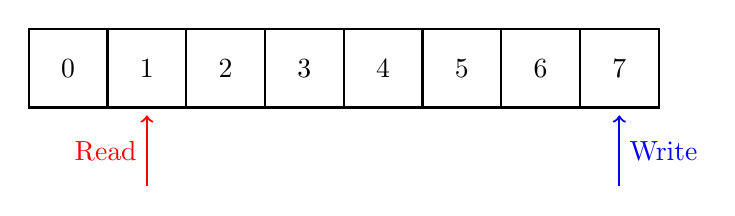
\begin{tikzpicture}
\foreach \i in {0,1,2,3,4,5,6,7} {
      \draw[thick] (\i,0) rectangle (\i+1,1); % Draw each spot in the queue
      \node at (\i+0.5, 0.5) {\i}; % Label each spot
}
\draw[thick, ->, red] (1.5, -1) -- (1.5, -0.1) node[midway, left] {Read};
\draw[thick, ->, blue] (7.5, -1) -- (7.5, -0.1) node[midway, right] {Write};
\end{tikzpicture}
\end{center}

Since the reader and writer execute in different contexts, the instructions in a read
and write can interleave in \textit{any} way imaginable:
\begin{itemize}
      \item Reader empty check can happen just as the writer is writing data
      \item Writer full check can happen just as the reader is reading data
      \item Reading and writing can occur concurrently
\end{itemize}

The key observation is the index held by the write pointer is reserved by the
writer. Similarly, the index held by the read pointer is reserved by the reader. The
only exception is when the read pointer equals to write pointer, then the queue is
empty. Given the possible ways the reader and writer execution can interleave, 
we can use TLA+ to verify the design.

\section{Specification}

% TLA+ specification can be written using its native formal specification language,
% or a C-like syntax called PlusCal (which transpires down to its native form).
% In this example, I chose to implement the specification using PlusCal, since the
% content to be verified is pseudo implementation. While it is possible to specify
% SPSC in native TLA+, I find the approach more error-prone as each line is
% effectively an individual state to be modeled.\\

The following is a snippet of the specification written in PlusCal:\\
\begin{ppcal}
procedure reader()
begin
r_chk_empty:            
      if rptr = wptr then 
      r_early_ret:                  
            return;
      end if;
r_read_buf:             
      assert buffer[rptr] # 0;
r_cs:                      
      buffer[rptr] := 0;
r_upd_rtpr:             
      rptr := (rptr + 1) % N;
      return;
end procedure; 
\end{ppcal}
\begin{tlatex}
\@x{ {\p@procedure} reader ( )}%
\@x{ {\p@begin}}%
\@x{ r\_chk\_empty\@s{.5}\textrm{:}\@s{3}}%
\@x{\@s{24.59} {\p@if} rptr \.{=} wptr {\p@then}}%
\@x{\@s{24.59} r\_early\_ret\@s{.5}\textrm{:}\@s{3}}%
\@x{\@s{49.19} {\p@return} {\p@semicolon}}%
\@x{\@s{24.59} {\p@end} {\p@if} {\p@semicolon}}%
\@x{ r\_read\_buf\@s{.5}\textrm{:}\@s{3}}%
\@x{\@s{24.59} {\p@assert} buffer [ rptr ] \.{\neq} 0 {\p@semicolon}}%
\@x{ r\_cs\@s{.5}\textrm{:}\@s{3}}%
\@x{\@s{24.59} buffer [ rptr ] \.{:=} 0 {\p@semicolon}}%
\@x{ r\_upd\_rtpr\@s{.5}\textrm{:}\@s{3}}%
\@x{\@s{24.59} rptr \.{:=} ( rptr \.{+} 1 ) \.{\%} N {\p@semicolon}}%
\@x{\@s{24.59} {\p@return} {\p@semicolon}}%
\@x{ {\p@end} {\p@procedure} {\p@semicolon}}%
\end{tlatex}
\\

The reader checks if the queue is empty by comparing the read and write pointers. If 
the queue is empty, reader early returns. If the queue is not empty, the reader reads the
index and advances the read pointer.\\
\begin{ppcal}
procedure writer() 
begin
w_chk_full:             
      if (wptr + 1) % N = rptr then 
      w_early_ret:
            return; 
      end if;
w_write_buf:
      assert buffer[wptr] = 0;
w_cs:
      buffer[wptr] := wptr + 1000;
w_upd_wptr:
      wptr := (wptr + 1) % N;
      return;
end procedure; 
\end{ppcal}\newline
\begin{tlatex}
\@x{ {\p@procedure} writer ( )}%
\@x{ {\p@begin}}%
\@x{ w\_chk\_full\@s{.5}\textrm{:}\@s{3}}%
\@x{\@s{24.59} {\p@if} ( wptr \.{+} 1 ) \.{\%} N \.{=} rptr {\p@then}}%
\@x{\@s{24.59} w\_early\_ret\@s{.5}\textrm{:}\@s{3}}%
\@x{\@s{49.19} {\p@return} {\p@semicolon}}%
\@x{\@s{24.59} {\p@end} {\p@if} {\p@semicolon}}%
\@x{ w\_write\_buf\@s{.5}\textrm{:}\@s{3}}%
\@x{\@s{24.59} {\p@assert} buffer [ wptr ] \.{=} 0 {\p@semicolon}}%
\@x{ w\_cs\@s{.5}\textrm{:}\@s{3}}%
\@x{\@s{24.59} buffer [ wptr ] \.{:=} wptr \.{+} 1000 {\p@semicolon}}%
\@x{ w\_upd\_wptr\@s{.5}\textrm{:}\@s{3}}%
\@x{\@s{24.59} wptr \.{:=} ( wptr \.{+} 1 ) \.{\%} N {\p@semicolon}}%
\@x{\@s{24.59} {\p@return} {\p@semicolon}}%
\@x{ {\p@end} {\p@procedure} {\p@semicolon}}%
\end{tlatex}
\\

The writer checks if the queue is full checking if there's more space to write
to. If the queue is full, the writer early exists. If the queue is not full, a writer
writes to the queue and advances the write pointer.\\

The key insight here is the read and write pointer effectively \textit{reserves}
the index they are pointing to. The state of the indices is unknown to the other
context. Assume a reader index of k, the writer cannot write to index k since
the reader might be reading from it. The only time a writer can write to k is
when the read index is no longer k, suggesting the reader is done with the
index. Symmetrically reasoning applies with the write index.

\section{Safety}

A correctness property for a lockless algorithm is to ensure reader and writer
cannot access the same index at the same time. Both reader and writer can be
working inside their critical section, but they \textit{cannot} be
working on the same index. The following formula describes this safety property:\\

\begin{tla}
MutualExclusion ==
      ~ ((pc[WRITER] = "w_cs") 
      /\ (pc[READER] = "r_cs") 
      /\ rptr = wptr)
\end{tla}
\begin{tlatex}
\@x{ MutualExclusion \.{\defeq}}%
\@x{\@s{24.59} {\lnot} ( ( pc [ WRITER ] \.{=}\@w{w\_cs} )}%
\@x{\@s{24.59} \.{\land} ( pc [ READER ] \.{=}\@w{r\_cs} )}%
\@x{\@s{24.59} \.{\land} rptr \.{=} wptr )}%
\end{tlatex}

\section{Liveness}

For liveness, we want to check the queue never hangs. This can be described as 
all indices are eventually used and unused:\\

\begin{tla}
Liveness ==
      /\ \A k \in 0..N-1:
            buffer[k] # 0 ~> buffer[k] = 0
      /\ \A k \in 0..N-1:
            buffer[k] = 0 ~> buffer[k] # 0
\end{tla}
\begin{tlatex}
\@x{ Liveness \.{\defeq}}%
\@x{\@s{24.59} \.{\land} \A\, k \.{\in} 0 \.{\dotdot} N \.{-} 1 \.{:}}%
\@x{\@s{24.59} buffer [ k ] \.{\neq} 0 \.{\leadsto} buffer [ k ] \.{=} 0}%
\@x{\@s{24.59} \.{\land} \A\, k \.{\in} 0 \.{\dotdot} N \.{-} 1 \.{:}}%
\@x{\@s{24.59} buffer [ k ] \.{=} 0 \.{\leadsto} buffer [ k ] \.{\neq} 0}%
\end{tlatex}

% \end{document}
